\documentclass[11pt]{homework}

\usepackage{tikz}
\usetikzlibrary{arrows,shapes,calc,positioning}
\usepackage{courier}
\def\defaultHypSeparation{\hskip 0.1in}
\usepackage{listing}
\lstset{
	basicstyle=\footnotesize\ttfamily,
	numbers=left,
	stepnumber=1,
	mathescape=true	
}

% TODO: replace these with your information
\newcommand{\hwname}{Chiao Hsieh}
\newcommand{\hwemail}{chsieh16@illinois.edu}
\newcommand{\hwtype}{Homework}
\newcommand{\hwnum}{I}
\newcommand{\hwclass}{CS 426: Compiler Construction}
\newcommand{\hwlecture}{}
\newcommand{\hwsection}{}

\renewcommand{\questiontype}{Problem}
\newcommand{\TT}{\ensuremath{\mathtt{true}}}
\newcommand{\FF}{\ensuremath{\mathtt{false}}}

\begin{document}
\maketitle

% Your content

\question
(\textit{50 points.}) Intermediate representations:

\begin{enumerate}[label=(\alph*)]

\item
Ans.

CFG for code fragment 2

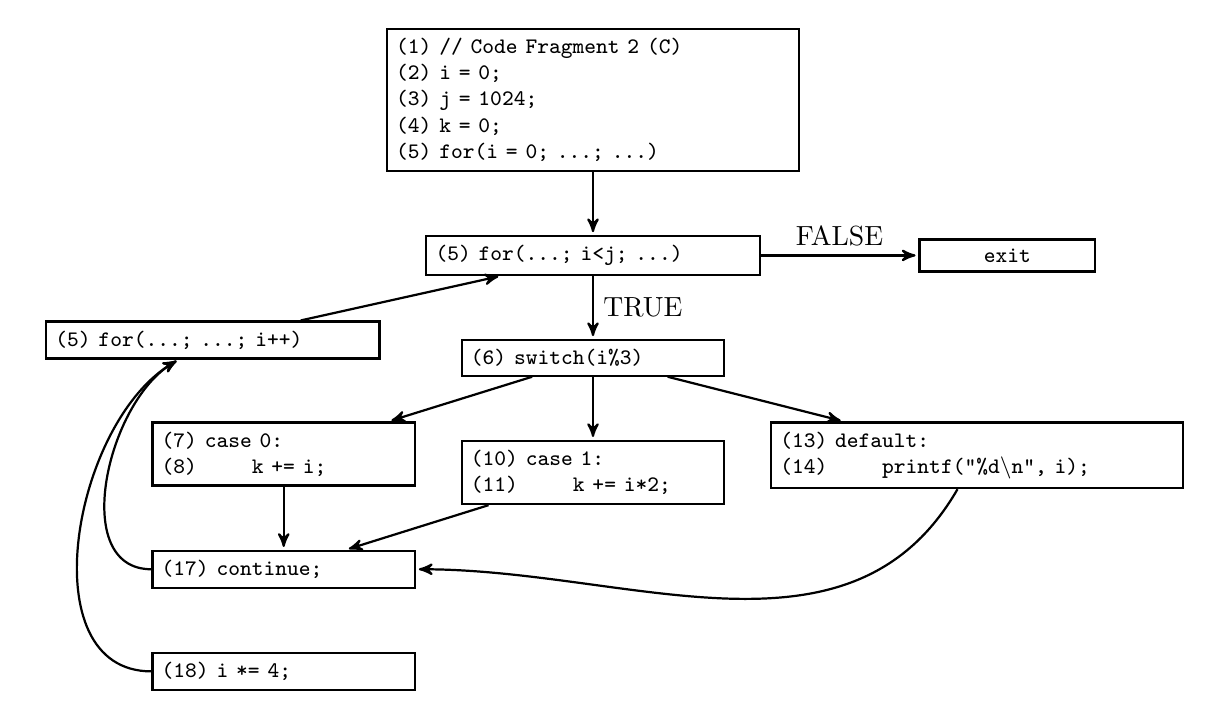
\begin{tikzpicture}[->,>=stealth',shorten >=1pt,auto,node
      distance=.8cm,thick,
      node/.style={rectangle,draw,minimum width=0.8cm, text width=3.1cm, font=\footnotesize\ttfamily}]

	\node[node, text width=5cm] (1) {
		(1) // Code Fragment 2 (C) \\
		(2) i = 0;\\
		(3) j = 1024;\\
		(4) k = 0;\\
		(5) for(i = 0; ...; ...)
	};
	
	\node[node, below=of 1, text width=4cm] (5-2) {
		(5) for(...; i<j; ...)
	};
	
	\node[node, below left=of 5-2, text width=4cm] (5-3) {(5) for(...; ...; i++)};
		
	\node[node, below=of 5-2] (6) {
		(6) switch(i\%3)
	};
	
	\node[node, below left=of 6] (7) {
		(7) case 0:\\
		(8) \qquad k += i;
	};
	
	\node[node, below=of 6] (10) {
		(10) case 1:\\
		(11) \qquad k += i*2;
	};

	\node[node, below right=of 6, text width=5cm] (13) {
		(13) default:\\
		(14) \qquad printf("\%d\textbackslash n", i);
	};
	
	\node[node, below=of 7] (17){ (17) continue;};

	\node[node, below=of 17] (18){ (18) i *= 4;};
	
	\node[node, text width=2cm, right=2cm of 5-2, align=center] (exit) {exit};

	\path
		(1) edge (5-2)
		(5-2) edge node [right] {TRUE} (6)
		(5-2) edge node [above] {FALSE} (exit)
		(5-3) edge (5-2)
		(6) edge (7)
		(6) edge (10)
		(6) edge (13)
		(7) edge (17)
		(10) edge (17)
		(13) [out=-120, in=0] edge (17)
		(17) [out=180, in=-150] edge (5-3)
		(18) [out=180] edge (5-3)
	;
\end{tikzpicture}

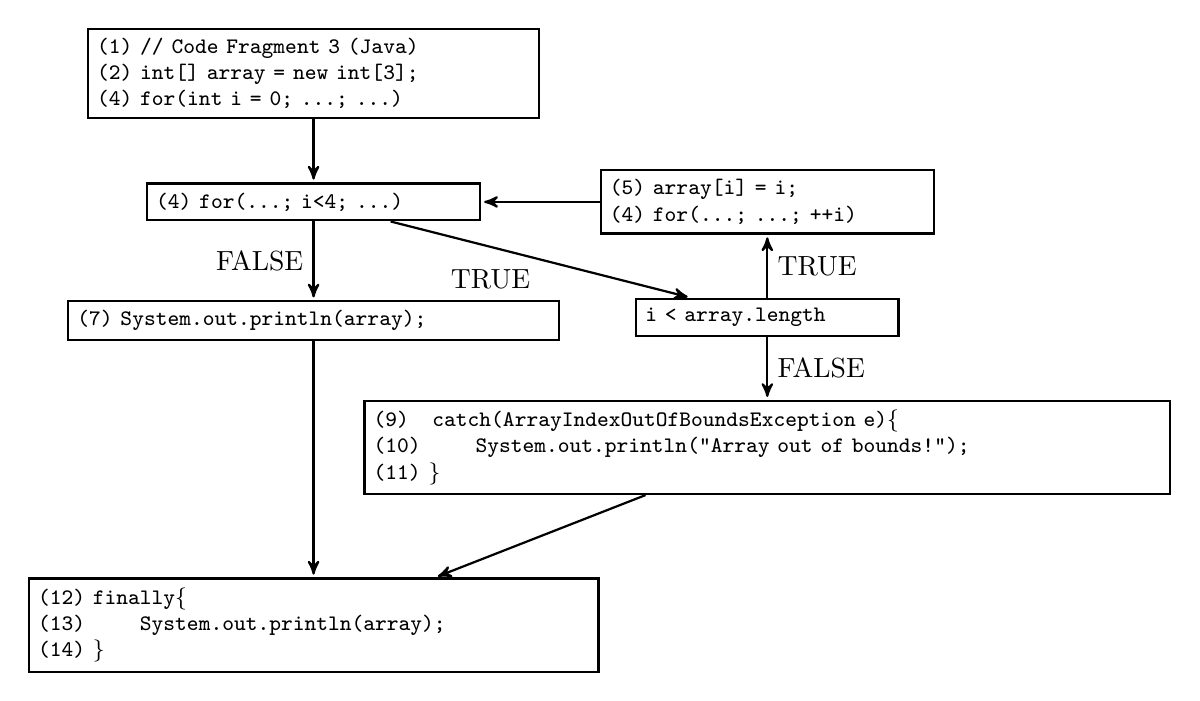
\begin{tikzpicture}[->,>=stealth',shorten >=1pt,auto,node
      distance=.8cm,thick,
      node/.style={rectangle,draw,minimum width=0.8cm, text width=3.1cm, font=\footnotesize\ttfamily}]

	\node[node, text width=5.5cm] (1) {
		(1) // Code Fragment 3 (Java) \\
		(2) int[] array = new int[3];\\
		(4) for(int i = 0; ...; ...)
	};
	
	\node[node, below=of 1, text width=4cm] (4-2) {
		(4) for(...; i<4; ...)
	};

	\node[node, right=1.5cm of 4-2, text width=4cm] (5) {
		(5) array[i] = i;\\
		(4) for(...; ...; ++i)
	};
		
	\node[node, below=of 5] (bound) {
		i < array.length
	};
	
	\node[node, below=1cm of 4-2, text width=6cm] (7) {
		(7) System.out.println(array);
	};
	
	\node[node, below=of bound, text width=10cm] (9) {
		(9)\ \ \ catch(ArrayIndexOutOfBoundsException e)\{\\
		(10) \qquad System.out.println("Array out of bounds!");\\
		(11) \}
	};
	\node[node, below=3cm of 7, text width=7cm] (12) {
		(12) finally\{\\
		(13) \qquad System.out.println(array);\\
		(14) \}
	};	

	\path
		(1) edge (4-2)
		(4-2) edge node [below left] {TRUE} (bound)
		(4-2) edge node [left] {FALSE} (7)
		(bound) edge node [right] {TRUE} (5)
		(bound) edge node [right] {FALSE} (9)
		(5) edge (4-2)
		(7) edge (12)
		(9) edge (12)
	;
\end{tikzpicture}

\item

Ans.

We first construct CFG of Code Fragment 1.

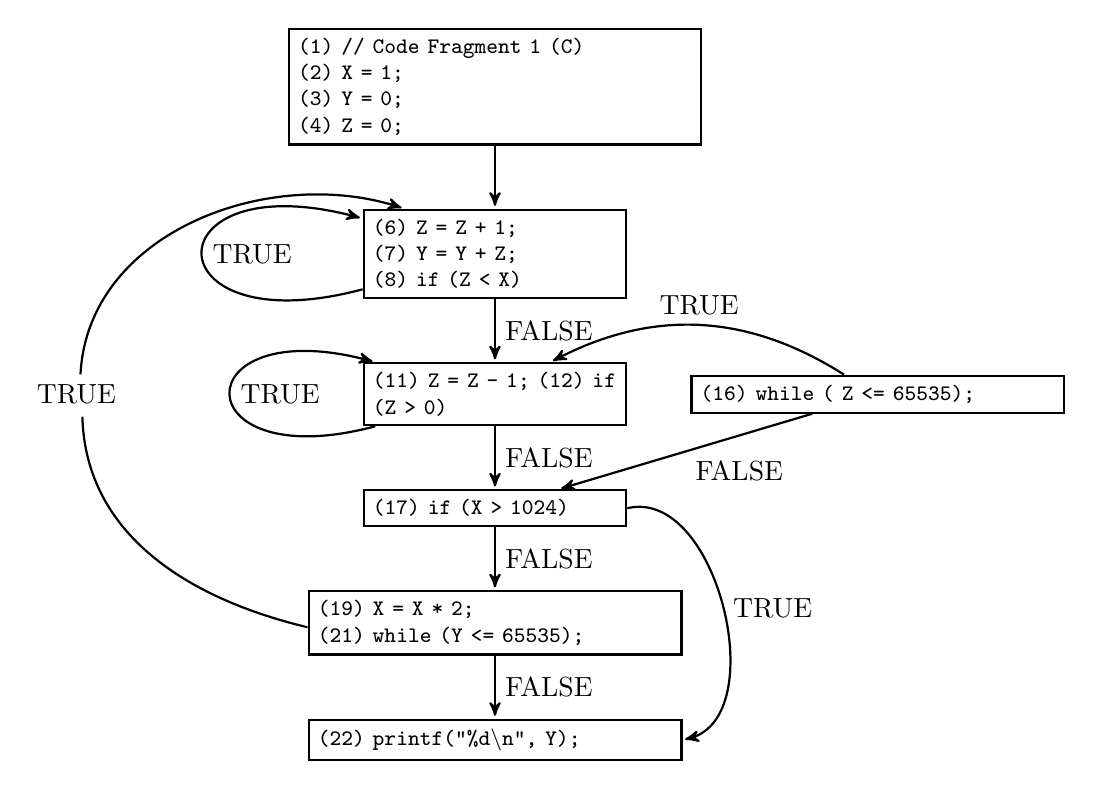
\begin{tikzpicture}[->,>=stealth',shorten >=1pt,auto,node
      distance=.8cm,thick,
      node/.style={rectangle,draw,minimum width=0.8cm, text width=3.1cm, font=\footnotesize\ttfamily}]

	\node[node, text width=5cm] (1) {
		(1) // Code Fragment 1 (C) \\
		(2) X = 1; \\
		(3) Y = 0; \\
		(4) Z = 0;
	};
	
	\node[node, below=of 1] (6) {
		(6) Z = Z + 1; \\
		(7) Y = Y + Z; \\
		(8) if (Z < X) 
	};
	
	\node[node, below=of 6] (11) {
		(11) Z = Z - 1;
		(12) if (Z > 0)
	};
	
	\node[node, text width=4.5cm, right=of 11] (16) {(16) while ( Z <= 65535);};
	
	\node[node, below=of 11] (17) {(17) if (X > 1024)};

	\node[node, text width=4.5cm, below=of 17] (19) {
	(19) X = X * 2; \\
	(21) while (Y <= 65535);
	};
	
	\node[node, text width=4.5cm, below=of 19] (22) {(22) printf("\%d\textbackslash n", Y);};

	\node [left=3cm of 11] (mid) {TRUE};

	\path
		 (1) edge (6)
		 (6) edge node [right] {FALSE} (11)
		(11) edge node [right] {FALSE} (17)
		(16) edge node [below right] {FALSE} (17)
		(17) edge node [right] {FALSE} (19)
		(19) edge node [right] {FALSE} (22)
		(16) [bend right] edge node [above] {TRUE} (11)
		(19) [out=30, in=135,-] edge (mid)
		(mid)[out=60,->] edge (6)
		(17) [out=90, in=90] edge node [right] {TRUE} (22)
	;
	\path
		 (6) [loop left] edge node [right] {TRUE} (6)
		(11) [loop left] edge node [right] {TRUE} (11)
	;
\end{tikzpicture}

From above, we derive SSA form of Code Fragment 1.
\begin{figure}
\begin{lstlisting}[language=C]
// Code Fragment 1 (C) SSA form
$X_0$ = 1;
$Y_0$ = 0;
$Z_0$ = 0;
do {
	$X_1$ = $\phi(X_0, X_2)$;
	$Y_1$ = $\phi(Y_0, Y_2)$;
	$Z_1$ = $\phi(Z_0, Z_4)$;
	$Z_2$ = $Z_1$ + 1;
	$Y_2$ = $Y_1$ + $Z_2$;
	if ($Z_2$ < $X_1$)
		continue;
	do {
		$Z_3$ = $\phi(Z_2, Z_4)$;
		$Z_4$ = $Z_3$ - 1;
		if ($Z_4$ > 0)
			continue;
		break;    // exits innermost do ... while loop
	}
	while ( Z <= 65535);
	if ($X_1$ > 1024)
		break;    // exits innermost do ... while loop
	$X_2$ = $X_1$ * 2;
}
while ($Y_2$ <= 65535);
printf("%d\n", $Y_2$);
\end{lstlisting}

\begin{lstlisting}[language=C]
// Code Fragment 2 (C)
$i_0$ = 0;
$j_0$ = 1024;
$k_0$ = 0;
$i_1$ = 0; // for(i = 0; i < j; ++i){
S:	$i_2$ = $\phi(i_1, i_4)$;
	$k_2$ = $\phi(k_0, k_5)$;
	if ($i_2$ >= $j_0$)
		goto E;
	switch($i_2$%3) {
		case 0:
			$k_3$ = $k_2$ + $i_2$;
			break;
		case 1:
			$k_4$ = $k_2$ + $i_2$*2;
			break;
		default:
			printf("%d\n", $i_2$);
			break;
	}
	$k_5$ = $\phi(k_2, k_3, k_4)$; goto INCRE;
	$i_3$ = i * 4 // i *= 4;
INCRE:	$i_4$ = $\phi(i_2, i_3)$;
	$i_5$ = $i_4$ + 1;
	goto S;
E:	;
\end{lstlisting}
\end{figure}

\end{enumerate}

\question


Ans.

\texttt{
\begin{tabular}[h]{l|l|l}
\textbf{Objects} & \textbf{Memory Region} & \textbf{Creation Time} \\
\hline
int Size    & Initialized Globals & Load Time \\
double GlobalStore[] & Uninitialized Globals & Load Time \\
void dummy(...) & Code & Link Time \\
struct Bag* B & Stack & Function Entry \\
int N & Stack & Function Entry \\
static double SaveSum & Initialized Globals & Load Time \\
int i & Stack & Function Entry \\
double x & Stack & Function Entry \\
double(*fp)(double) & Stack & Function Entry \\
struct Contents* listS & Stack & Function Entry \\
struct Contents* nextSPtr & Stack & Function Entry \\
struct Contents* nextHPtr & Stack & Function Entry \\
(*listS) /* Object1 */ & Stack & Statement Runtime \\
struct Contents *ptr; & Stack & Function Entry \\
(*ptr) /* Objects2 */ & Heap & Statement Runtime \\
(*ptr) /* Objects3 */ & Stack & Statement Runtime \\
\end{tabular}
}

\question
\begin{enumerate}[label=(\alph*)]
\item The numbers and types of arguments for a method \\
      Ans. Static Type
\item The address of the function to call \\
      Ans. Dynamic Type
\item The vtable to use for the call \\
      Ans. Dynamic Type
\item The offset (or field index in LLVM) of the vtable pointer within the object struct \\
      Ans. Static Type
\item The offset (or field index in LLVM) of the function pointer entry within the vtable struct \\
      Ans. Static Type
\item The number of load instructions that must be executed before making the call \\
      Ans. Neither
\end{enumerate}

\question
\begin{enumerate}[label=(\alph*)]
\item Assign address range for a global variable. \\
      Ans. At compile time 
\item Compute address of a local variable. \\
      Ans. At compile time
\item Encounter a shift-reduce conflict. \\
      Ans. At compiler construction time
\item Choose in which area of memory (static data, heap, or stack) a particular variable will be stored. \\
      Ans. At compile time
\item In a language with strong type safety (like Java), check that the type of an operand can be correctly converted (i.e., type-cast) to the type of the result variable for a particular operation. \\
      Ans. At compile time if up-cast to base type.
      Runtime if down-cast to derived type.
\item Allocate storage for an activation record. \\
      Ans. At compile time if the programming language doesn't allow variable size local variables such as array with variable length.
      At run-time, otherwise.

\end{enumerate}

\end{document}